\section{Development of the Control Application}
\label{sec:control_sw}
Control software was developed to ease testing of the stepper motor controller functionality.
The control software was also developed in the Rust programming language, utilizing a crate for \acs{tui} (\acl{tui}) and the shared components library from the bare-metal firmware.
Initially, we aimed to develop a fully-featured \acs{gui} (\acl{gui}) based on the GTK framework, but this work hasn't left the prototyping stage as the learning curve for integrating GTK is quite steep.
In the Figure~\ref{fig:tui} we can see the control application, and in the Figure~\ref{fig:gui}, there is a screenshot of the proposed \acs{gui} developed with the GTK framework.

\begin{figure}[H]
    \centering
    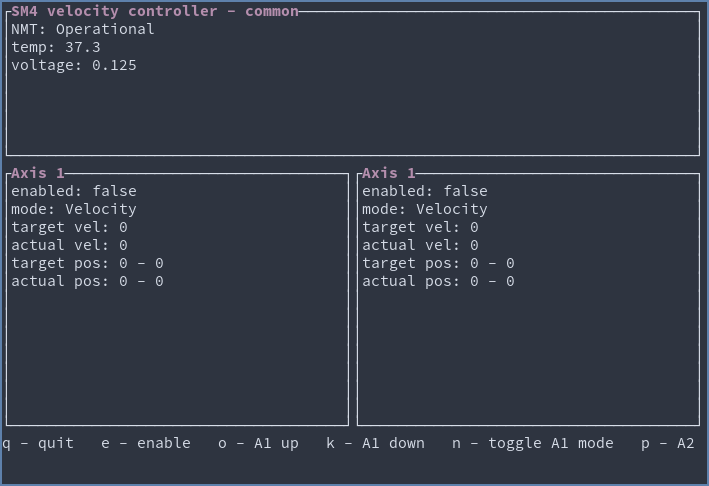
\includegraphics[width=0.8\textwidth]{obrazky/tui}
    \caption{The TUI control application.}
    \label{fig:tui}
\end{figure}

\begin{figure}[H]
    \centering
    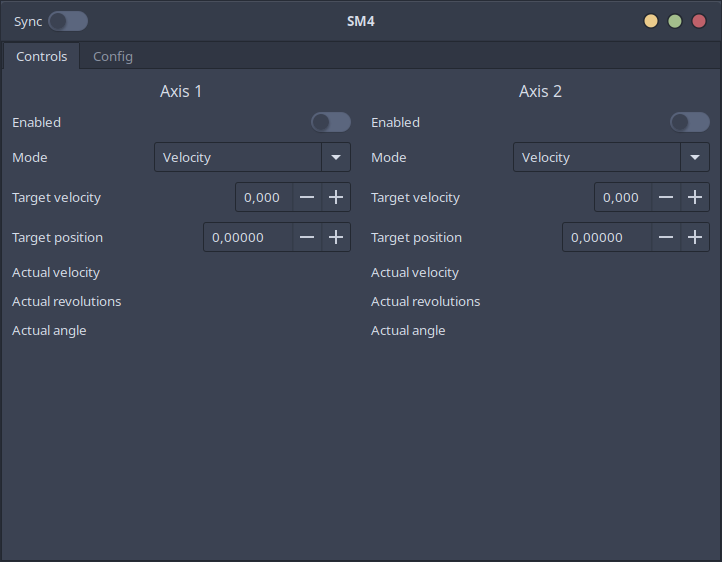
\includegraphics[width=0.8\textwidth]{obrazky/gui}
    \caption{The proposed GUI control application.}
    \label{fig:gui}
\end{figure}


For communication with the stepper motor controller, the control application utilizes CANOpen protocol.
It periodically transmits \textbf{SYNC} frames and displays the contents of the received \textbf{PDO}s.
On various keypresses, it changes the values of the control variables (such as axis target velocity and target position) and sends them to the controller.
This way, it can be easily tested whether the controller works as expected.

In the future, apart from developing a proper \acs{gui} for the control application, we want to add support for all the remaining communication interfaces and configuring all the parameters of the stepper motor controller.
